\chapter{Scania C300 Communicator} \label{rtc-c300}
% The communicator contains iMX6 series processors

Scania ECU was set to be the target hardware to benchmark the training of a machine learning model. The ECU is developed by an external system maker Actia who designed the board in association with Scania and with an i.MX6 series processor and a number of on-board peripherals including CAN controllers. Much of the build system configuration files and Yocto BSP layers used for the board are not made available by the system maker, instead providing embedded Linux binaries and SDKs to Scania. The initial mandate included creating such a BSP layer for the C300 which would facilitate the repurposing of the hardware on board. For this purpose, some examinations on the board were conducted and this part of the report will account the activites made in this effort.

\begin{figure}[h]
	\centering
	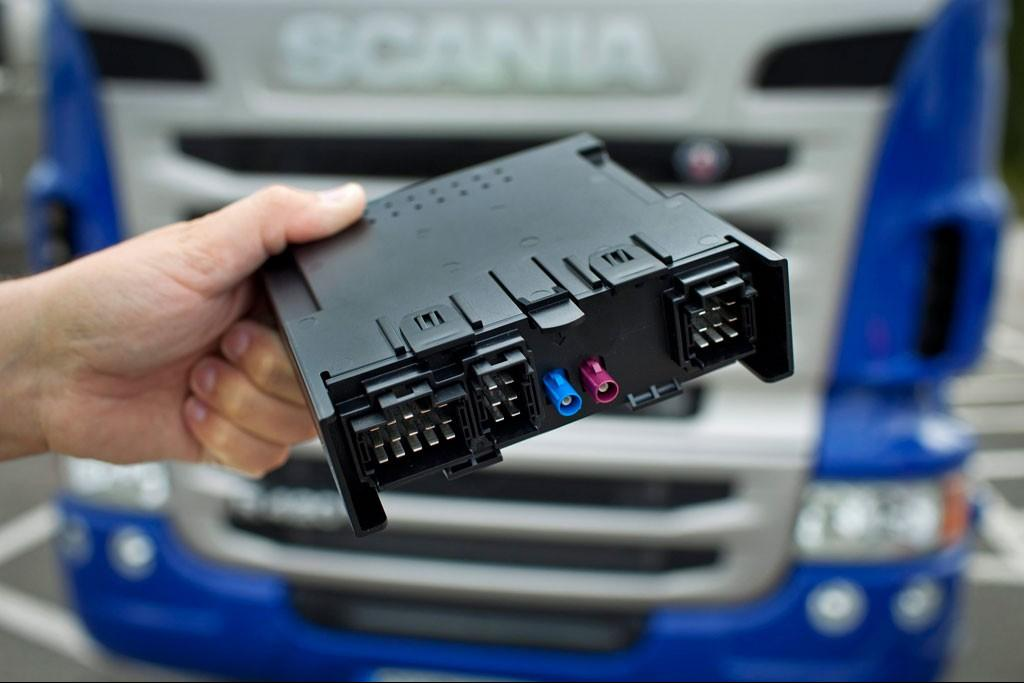
\includegraphics[scale=0.34]{c300.jpeg}
\end{figure}

\subsubsection*{Development Tools}

The U-Boot bootloader on a vanilla C300 is silent. The documentation contained little information on the device tree and no memory layout information. The boot flow information of the processor was available from NXP but no information was available on any modifications made by the system vendor. The lack of these resources made it difficult to port or install any tool/package on the device to reveal certain basic information. The information that was available about the processor were the number of cores, the instruction set architecture, the supported memory units, and the basic kernel information from the name, version, and distribution. There was visibility into the file system however, and to the presence of the bootloader code as well

% Research and experiments conducted on the Scania ECU to reverse engineering and obtain the required hardware and software information . Further, repurposing the ECU by flashing a custom operating system to benchmark the neural network applications was also attempted.

% The efforts were conducted both when the ECU started up in its usual operation and when it was booted in serial download mode.

\subsubsection*{Approach}

The first naive approach taken was of flashing the MTD partitions that houses the bootloader. This was to verify that it is possible to flash the same bootloader and to then boot the board. A dump of the existing bootloader was taken and flashed in the same partition. This worked and the device booted successfully. Next, the u-boot bootloader developed from the yocto project was flashed on the bootloader MTD partition with the little device information that was available and sample by examing the board. However the broad was bricked, pressumably due to the u-boot image having incomplete or wrong device tree structure or perhaps the loading kernel failed as version mismatch between bootloader and kernel, or a checksum failure, or perhaps the size of the file was big enough to overwrite a different crucial region.

% (TODO: Using mfgtools on board, to collect information from bootloader.)
% (TODO: Using uuu tool in SDM mode to flash custom image.)
% (TODO: bootloader flashing using dd command)

% (TODO: results from varying bootloader environment parameters)
% (TODO: results from mfgtools experiment)
% (TODO: results of unbricking the board)
% (TODO: reasoning not enough memory layout infomation)

Exploring the target ECU board involved several examinations of a known state of the board. The Linux kernel binaries were made via the Yocto project however there was no access to source code such as the recipes or the meta-layers themselves

The i.MX SoCs have a special boot mode named Serial Download Mode (SDM) typically accessible through boot switches. When configured into this mode, the ROM code will poll for a connection on a USB OTG port
